% Full instructions available at:
% https://github.com/elauksap/focus-beamertheme

\documentclass{beamer}
\usepackage{pifont}
\usepackage{listings}
\usepackage{ulem}
\usetheme{focus}

\title{Recovering enzyme haplotypes from metagenomes}
% \subtitle{Subtitle}
\author{Girish Vyas \texorpdfstring{\\}{,} Dr. Wayne Aubrey}
% \author{Girish Vyas}

% \titlegraphic{\includegraphics[scale=1.25]{focuslogo.pdf}}
\institute{Aberystwyth University}

% \date{dd mm yyyy}

\begin{document}
\begin{frame}
	\maketitle
 gdv1@aber.ac.uk
\end{frame}

\section{Background}
\setbeamertemplate{caption}[numbered]
\begin{frame}[t]
	\begin{columns}
		\column{0.6\textwidth}
		\begin{figure}
			\centering
			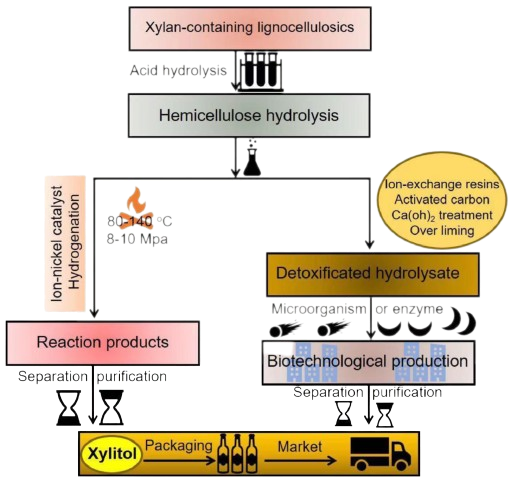
\includegraphics[width=\textwidth,height=0.4\textheight,keepaspectratio]{prod.png}
			\caption{Producing Xylitol \cite{xuBiosyntheticStrategiesProduce2019}}
		\end{figure}
		\begin{itemize}
			\item A sugar-substitute alditol
			\item Chemical \ding{55} Biotechnological \ding{51}
			\item Need to find enzymes for increasing yield
			\item XYL1: D-xylulose -> Xylitol
			\item Yeast: ~95\% C. Tropicalis: ~97\%
		\end{itemize}
		
		                
		\column{0.4\textwidth}
		\begin{figure}
			\centering
			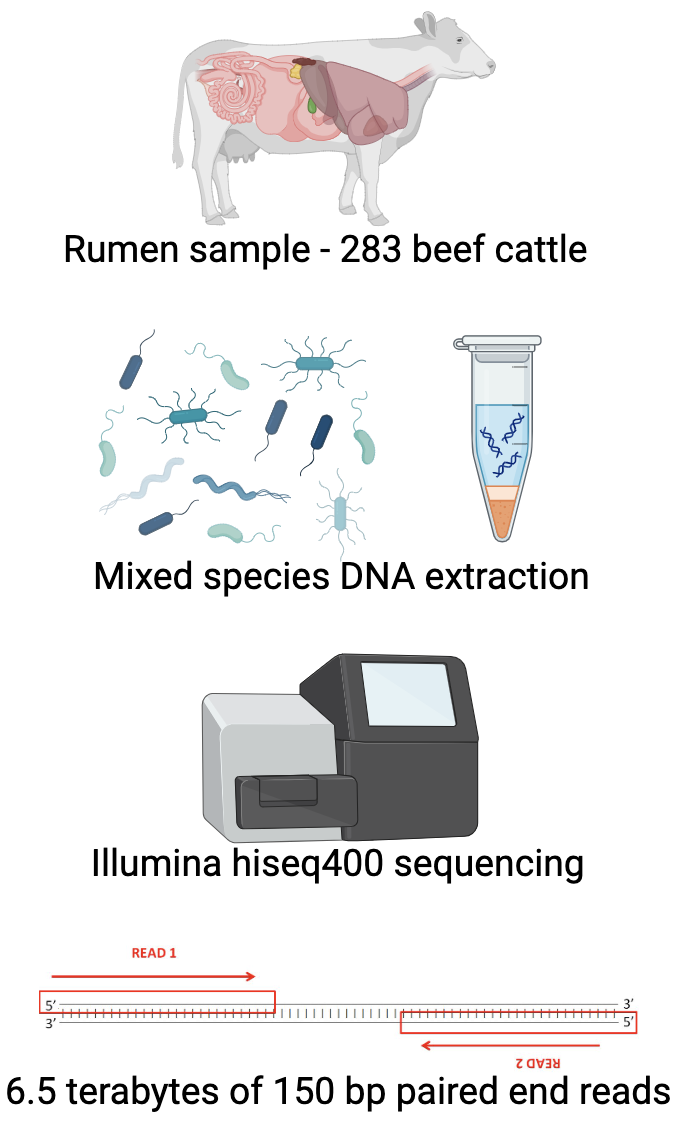
\includegraphics[width=\textwidth,height=0.8\textheight,keepaspectratio]{hyngate_workflow.png}
			\caption{Hungate metagenome (by waa2@)}
		\end{figure}
		% \begin{itemize}
		% 	\item Study of uncultured microorganisms
		% 	\item Hungate: 150bp paired-end reads of cattle rumen
		% 	\item 69K proteins / 90\% unknown
		% \end{itemize}
		
		
		                
		                
	\end{columns}
\end{frame}

% \begin{frame}[t]
% 	\begin{columns}
% 		\column{0.6\textwidth}
% 		\begin{figure}
% 			\centering
% 			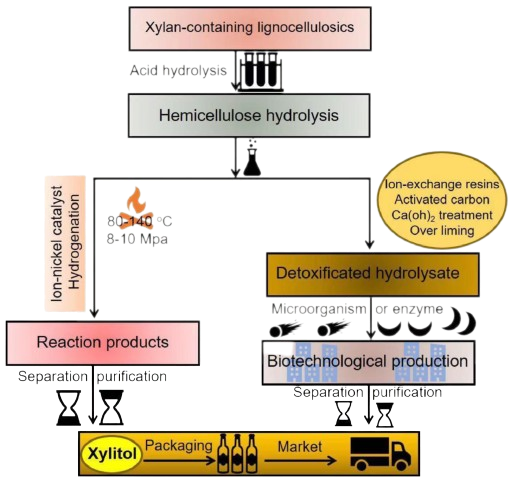
\includegraphics[width=\textwidth,height=0.4\textheight,keepaspectratio]{prod.png}
% 			\caption{Producing Xylitol \cite{xuBiosyntheticStrategiesProduce2019}}
% 		\end{figure}
% 		\begin{itemize}
% 			\item A sugar-substitute alditol
% 			\item Chemical \ding{55} Biotechnological \ding{51}
% 			\item Need to find enzymes for increasing yield
% 			\item XYL1: D-xylulose -> Xylitol
% 			\item Yeast: ~95\% C. Tropicalis: ~97\%
% 		\end{itemize}
		
		                
% 		\column{0.4\textwidth}
		
			
%    \scalebox{0.4}{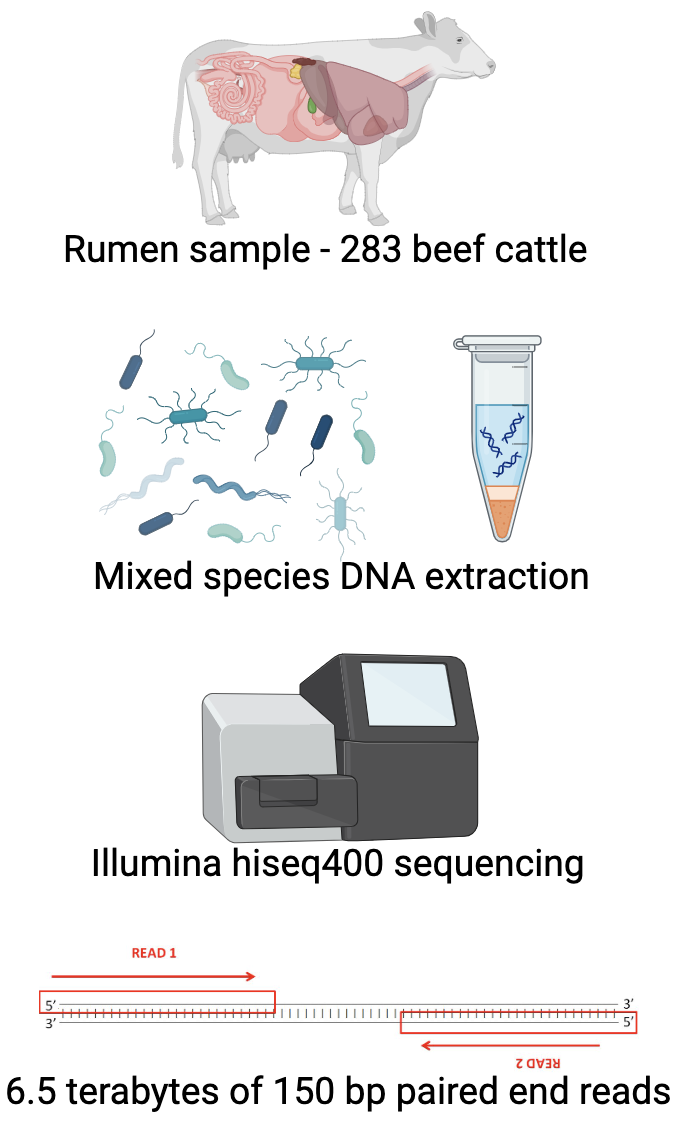
\includegraphics{hyngate_workflow.png}}
		       
% 	\end{columns}
% \end{frame}

\setbeamertemplate{caption}[numbered]
\begin{frame}[t]{}
	\begin{columns}
		\column{0.5\textwidth}
		\begin{itemize}
			\item DNA fragments read from both sides
			\item Specific to Illumina sequencing; allows better mapping of repetitive regions 
			\item Alleles (X) are variations (SNP's) present at specific locus
			\item Haplotypes are set of alleles $\{X, Y\}$ that tend to be inherited together
			\item Genotype: All the alleles $(\{X_1, Y_1\}, \{X_2, Y_2\})$
		\end{itemize}
		                
		\column{0.5\textwidth}
		\begin{figure}
			\centering
			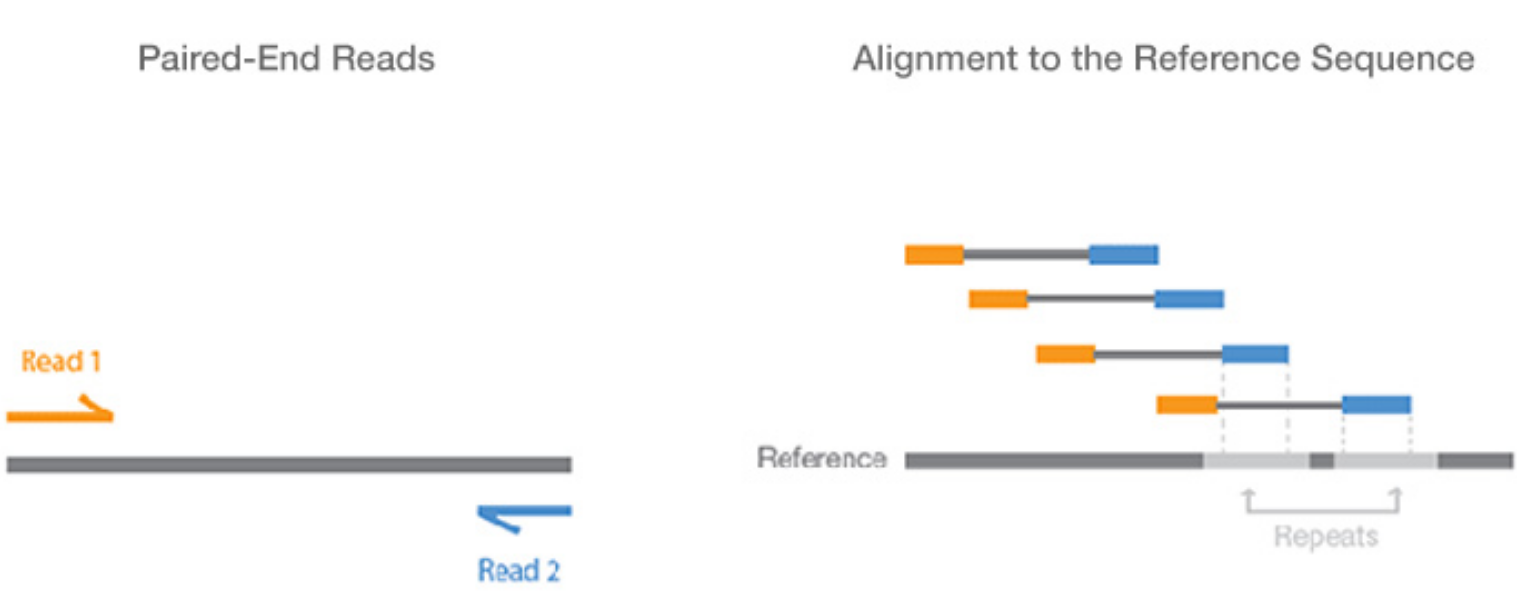
\includegraphics[width=\textwidth,height=0.3\textheight,keepaspectratio]{pairs.png}
			\caption{Paired reads \cite{PairedEndVsSingleRead}}
		\end{figure}
		\begin{figure}
			\centering
			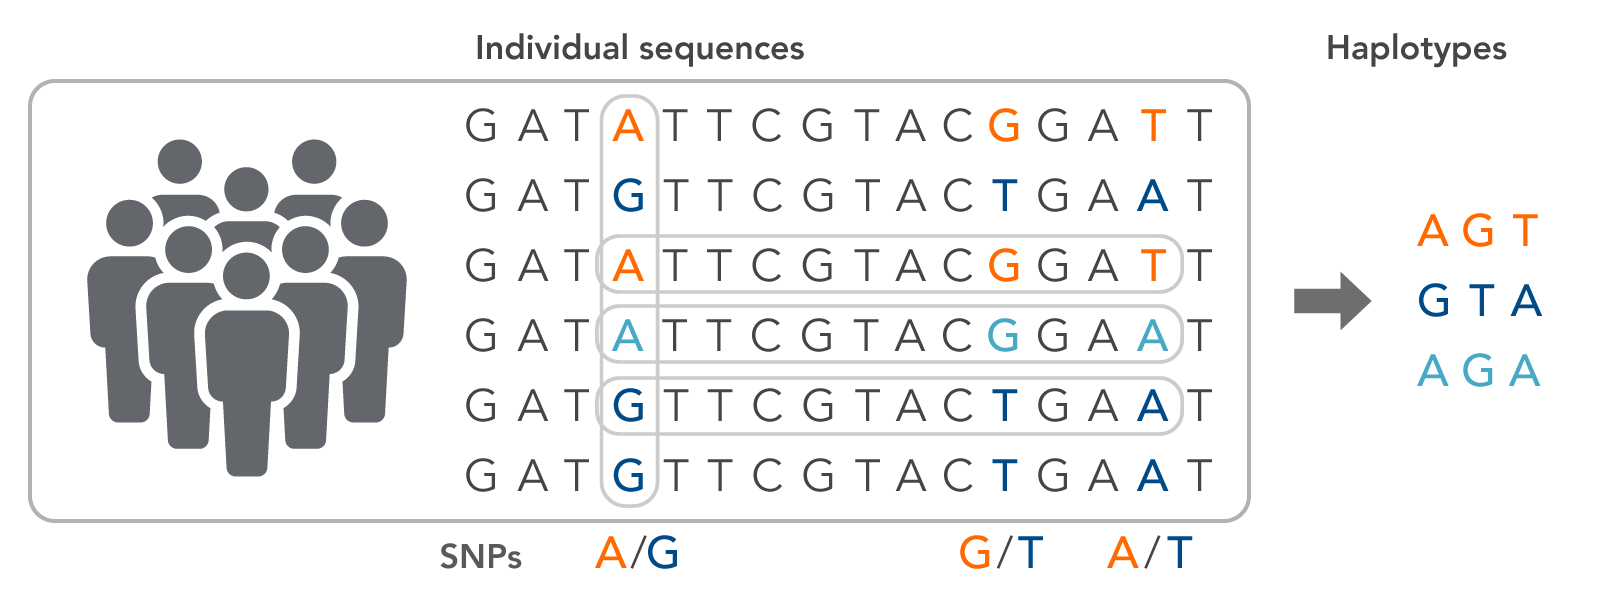
\includegraphics[width=\textwidth,height=0.5\textheight,keepaspectratio]{haplo.png}
			\caption{Haplotypes \cite{AlleleVsGenotype}}
		\end{figure}
	\end{columns}
\end{frame}


\section{Metagenomic SNP haplotyping pipeline}

\begin{frame}[fragile]
	\textbf{SIH Problem}: ``Given a set of fragments obtained by DNA sequencing from the two copies of a chromosome, reconstruct the two haplotypes from the SNPs values observed in the fragments.''\cite{lanciaSNPsProblemsComplexity2001} \\
	\textbf{MIH Problem}
	\begin{itemize}
		\item Cannot assume diploid
		\item Conflicting data cannot be verified due to varying ploidy
		\item Unknown number of haplotypes
	\end{itemize}
	\textbf{Enter Hansel\&Gretel}
	\begin{lstlisting}[language=bash]
gretel bam vcf contig --master reference
	\end{lstlisting}
	
\end{frame}

\begin{frame}[t]
	\begin{columns}
		\column{0.4\textwidth}
		\begin{itemize}
			\item \textbf{Alignment}
			      \begin{itemize}
			      	\item \textbf{Reference}: xylose reductase (xyl1) gene, complete cds
			      	\item \textbf{Choice}: blast (blastn, megablast, magicblast), bwa, bowtie2, minmap2
			      	\item \textbf{QC}: FastQC, Bloomine, Sourmash
			      	\item \textbf{Post-processing}: Binarize, Validation, Sorting, De-duplication, Merging
			      \end{itemize}
		\end{itemize}
		\column{0.6\textwidth}
		\begin{figure}
			\centering
			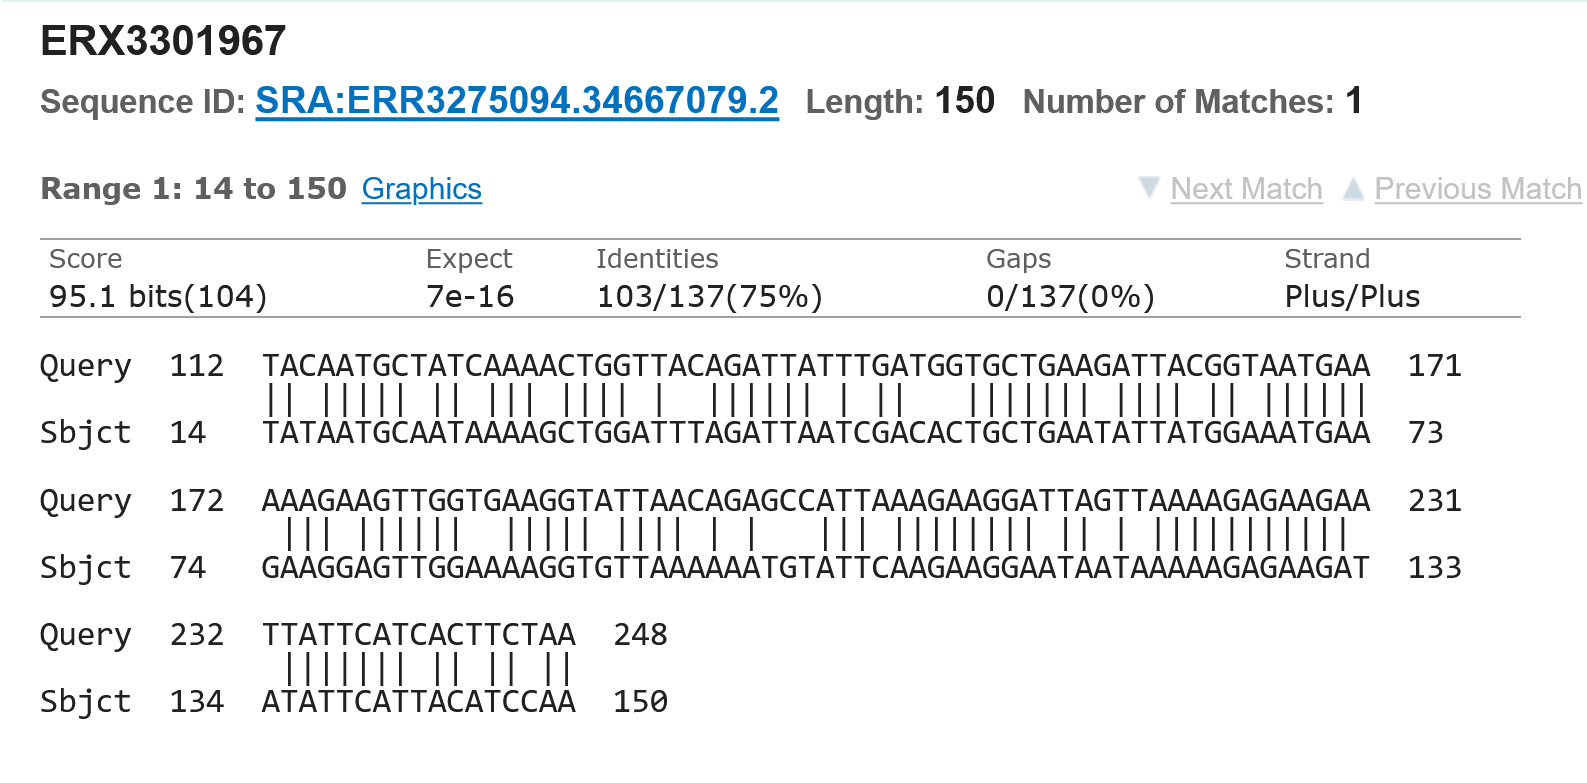
\includegraphics[width=\textwidth,height=0.5\textheight,keepaspectratio]{aln.png}
			\caption{Example Blast alignment}
		\end{figure}
		        
		        
	\end{columns}
	
\end{frame}

\begin{frame}[t]
	\begin{itemize}
		\item \textbf{Variant Calling}
		      \begin{itemize}
		      	\item \textbf{Choice}: bcftools, gatk, snpper.py
		      	\item \textbf{Post-processing}: bunzip compression, tabix
		      \end{itemize}
		                      
	\end{itemize}
	
	\begin{table}[!ht]
		\centering
		\begin{tabular}{|l|l|l|l|l|l|l|}
			\hline
			\textbf{\#CHROM} & \textbf{POS} & \textbf{ID} & \textbf{REF} & \textbf{ALT} & \textbf{QUAL} & \textbf{FILTER} \\ \hline
			AB540108.1       & 1579         & .           & C            & A            & 11.7172       & .               \\ \hline
			AB540108.1       & 1620         & .           & C            & T            & 11.7172       & .               \\ \hline
			AB540108.1       & 1662         & .           & G            & A            & 4.38466       & .               \\ \hline
			AB540108.1       & 1672         & .           & A            & G            & 11.7172       & .               \\ \hline
			AB540108.1       & 1686         & .           & T            & C            & 11.7172       & .               \\ \hline
			AB540108.1       & 1711         & .           & T            & C            & 11.7172       & .               \\ \hline
			AB540108.1       & 1736         & .           & T            & A            & 8.13869       & .               \\ \hline
			AB540108.1       & 1760         & .           & T            & C            & 11.7172       & .               \\ \hline
			AB540108.1       & 1773         & .           & T            & C            & 11.7172       & .               \\ \hline
			AB540108.1       & 1775         & .           & C            & T            & 11.7172       & .               \\ \hline
			MF045437.1       & 998          & .           & G            & A            & 11.7172       & .               \\ \hline
			MF045437.1       & 1011         & .           & A            & G            & 11.7172       & .               \\ \hline
		\end{tabular}
	\end{table}
\end{frame}

% \section{Workflow, Results \& Future Scope}
% \begin{frame}[t]
	    
% 	\begin{columns}
% 		\column{0.33\textwidth}
% 		\begin{itemize}
% 			\item \textbf{Workflow} Primary constraints: Processing 6.5T in 1.5T disk space
% 			\item Iteratively run 6-12 parallel jobs with following steps:
% 			      \begin{itemize}
% 			      	\item Check available space
% 			      	\item Prefetch sra archive
% 			      	\item Dump fastq files
% 			      	\item Run bowtie
% 			      \end{itemize}
% 		\end{itemize}
% 		\column{0.33\textwidth}
% 		\begin{itemize}
% 			\item \textbf{Results}
% 			      \begin{itemize}
% 			      	\item 1047 aligned reads
% 			      	\item 18 Variants
% 			      	\item 0 recovered haplotypes
% 			      	\item Completion time: ~4 days
% 			      \end{itemize}
% 		\end{itemize}
		
% 		\column{0.33\textwidth}
% 		\begin{itemize}
% 			\item \textbf{(Near) Future Scope}
% 			      \begin{itemize}
% 			      	\item Retry with more XYL1 genes
% 			      	\item Have some positive control by aligning to genes known to be present or MAG's
% 			      	\item Use a more sensitive alignment tool or tweak alignment parameters
% 			      \end{itemize}
% 		\end{itemize}
% 	\end{columns}
	
% \end{frame}

\begin{frame}{Workflow, Results}
	\item \textbf{Workflow}
 \begin{itemize}
 \item Primary constraints: Processing 6.5T in 1.5T disk space
			\item Iteratively run 6-12 parallel jobs with following steps:
			      
			      	\item Check available space
			      	\item Prefetch sra archive
			      	\item Dump fastq files
			      	\item Run bowtie
			      \end{itemize}
         
    \textbf{Results}
   \begin{itemize}
			      	\item 1047 aligned reads
			      	\item 18 Variants
			      	\item 0 recovered haplotypes
			      	\item Completion time: ~4 days
			    
		\end{itemize}
\end{frame}

\begin{frame}{Future Work}
\begin{itemize}
\item Have some positive control by aligning to genes known to be present or MAG's
\item Retry with other metagenomes (termite gut, moth gut, marine crustaceans wood-boring isopods gut.) 
\item Retry with more XYL1 genes
\item Use a more sensitive alignment tool or tweak alignment parameters
\end{itemize}
\end{frame}

\begin{frame}[focus]
	\sout{Questions} Suggestions?
\end{frame}
    
\appendix
\begin{frame}{References}
	\nocite{*}
	\bibliography{demo_bibliography}
	\bibliographystyle{plain}
\end{frame}
    
% \begin{frame}[t]
%     This frame has an empty title and is aligned to top.
% \end{frame}

    
    
% \begin{frame}[noframenumbering]{No frame numbering}
%     This frame is not numbered and is citing reference \cite{knuth74}.
% \end{frame}

    
    
%     \begin{frame}{Typesetting and Math}
%         The packages \texttt{inputenc} and \texttt{FiraSans}\footnote{\url{https://fonts.google.com/specimen/Fira+Sans}}\textsuperscript{,}\footnote{\url{http://mozilla.github.io/Fira/}} are used to properly set the main fonts.
%         \vfill
%         This theme provides styling commands to typeset \emph{emphasized}, \alert{alerted}, \textbf{bold}, \textcolor{example}{example text}, \dots
%         \vfill
%         \texttt{FiraSans} also provides support for mathematical symbols:
%         \begin{equation*}
%             e^{i\pi} + 1 = 0.
%         \end{equation*}
%     \end{frame}

%     \section{Section 2}
%     \begin{frame}{Blocks}
%         \begin{block}{Block}
%             Text.
%         \end{block}
%         \pause
%         \begin{alertblock}{Alert block}
%             Alert \alert{text}.
%         \end{alertblock}
%         \pause
%         \begin{exampleblock}{Example block}
%             Example \textcolor{example}{text}.
%         \end{exampleblock}
%     \end{frame}
    
%     \begin{frame}{Lists}
%         \begin{columns}[t, onlytextwidth]
%             \column{0.33\textwidth}
%                 Items:
%                 \begin{itemize}
%                     \item Item 1
%                     \begin{itemize}
%                         \item Subitem 1.1
%                         \item Subitem 1.2
%                     \end{itemize}
%                     \item Item 2
%                     \item Item 3
%                 \end{itemize}
            
%             \column{0.33\textwidth}
%                 Enumerations:
%                 \begin{enumerate}
%                     \item First
%                     \item Second
%                     \begin{enumerate}
%                         \item Sub-first
%                         \item Sub-second
%                     \end{enumerate}
%                     \item Third
%                 \end{enumerate}
            
%             \column{0.33\textwidth}
%                 Descriptions:
%                 \begin{description}
%                     \item[First] Yes.
%                     \item[Second] No.
%                 \end{description}
%         \end{columns}
%     \end{frame}
% \setbeamertemplate{caption}[numbered]
%     \begin{frame}{Figures and Tables}
%         \begin{columns}
%             \column{0.4\textwidth}
%                 \begin{figure}
%                     \centering
%                     \includegraphics{focuslogo.pdf}
%                     \caption{Figure caption.}
%                     \label{fig:focuslogo}
%                 \end{figure}
                
%             \column{0.6\textwidth}
%                 \begin{table}
%                     \centering
%                     \begin{tabular}{rcc}
%                          & Heading 1 & Heading 2 \\\hline
%                         Row 1 & \(v_{11}\) & \(v_{12}\) \\
%                         Row 2 & \(v_{21}\) & \(v_{22}\) \\
%                         Row 3 & \(v_{31}\) & \(v_{32}\) \\
%                     \end{tabular}
%                     \caption{Table caption.}
%                     \label{tab:demo}
%                 \end{table}
%         \end{columns}
%     \end{frame}
    
% \begin{frame}{Backup frame}
%     \usebeamercolor[fg]{normal text}
%     This is a backup frame, useful to include additional material for questions from the audience.
%     \vfill
%     The package \texttt{appendixnumberbeamer} is used not to number appendix frames.
% \end{frame}
\end{document}